

\chapter{Time Differencing Schemes}\label{ch:time-differencing-schemes}

In this chapter we consider ordinary differential equations with one
dependent and one independent variable. Although atmospheric models are
essentially always models for solving a complex set of partial
differential equations, in some formulations the numerical solution of
ordinary differential equations forms an important part of the
computational procedure. For instance in spectral models the governing
partial differential equations reduce to a set of ordinary differential
equations for the expansion coefficients as dependent variables. A set
of ordinary differential equations will also be obtained if a Lagrangian
method is used, in which the computational points move with the fluid.
But, most of all, schemes for solving ordinary differential equations
are of interest here since they are often used without modification to
construct approximations to the time derivative terms in the governing
partial differential equations. Knowledge of the properties of schemes
for solving ordinary differential equations will then be used in
investigating the properties of more complex schemes for solving the
partial differential equations.

With that in mind, we shall here first define some of the schemes that
will be interesting to analyze. Then we shall investigate the behaviour
of numerical solutions obtained when these schemes are used for two
specific ordinary differential equations: the oscillation (or frequency)
equation, and the friction equation. These equations will serve as
prototypes for later extension of the results to advection,
gravity-inertia wave, and diffusion processes within the atmospheric
primitive equations.

\section{Definitions of some schemes}\label{sec:def-some-schemes}

Schemes used for the time derivative terms within the primitive
equations are relatively simple, usually of the second and sometimes
even only of the first order of accuracy. There are several reasons for
this. First, it is a general experience that schemes
constructed so as to have a high order of accuracy are mostly not very
successful when solving partial differential equations. This is in
contrast to the experience with ordinary differential equations, where
very accurate schemes, such as the Runge-Kutta method, are extremely
rewarding. There is a basic reason for this difference. With an
ordinary differential equation, the equation and a single initial
condition is all that is required for an exact solution. Thus, the error
of the numerical solution is entirely due to the inadequacy of the
scheme. With a partial differential equation, the error of the numerical
solution is brought about both by the inadequacy of the scheme and by
insufficient information about the initial conditions, since they are
known only at discrete space points. Thus, an increase in the accuracy
of the scheme improves only one of these two components, and the results
are not too impressive.

Another reason for not requiring a scheme of high accuracy for
approximations to the time derivative terms is that, in order to meet a
stability requirement of the type discussed in the preceding chapter, it
is usually necessary to choose a time step significantly smaller than
that required for adequate accuracy. With the time step usually chosen,
other errors, for example in the space differencing, are much greater
than those due to the time differencing. Thus, computational effort is
better spent in reducing these other errors, and not in increasing the
accuracy of the time differencing. This, of course, does not mean that
it is not necessary to consider carefully the properties of various
possible time differencing schemes. Accuracy, is only one important
consideration in choosing a scheme.

To define some schemes, we consider the equation

\[\frac{\text{dU}}{\text{dt}} = f( U,t) \quad  U = U(t)\]

The independent variable t is here called time. We divide the time axis
into segments of equal length \(\Delta t\). We shall denote by
\(U^{\left( n \right)}\) the approximate value of U at time
\(n\Delta t\). We assume that we know at least the first of the values
\(U^{\left( n \right)}\), \(U^{\left( n - 1 \right)}\) \ldots and we want
to construct a scheme for computation of an approximate value
\(U^{\left( n + 1 \right)}\). These are many possibilities.

\subsection{Two level schemes}\label{subsec:two-level-schemes}

These are schemes that relate values of the dependent variable at two
time levels : n and n + 1. Only a two level scheme can be used to
advance an integration over the first time step, when just a single
initial condition is available. With such a scheme we want to
approximate the exact formula

\[U^{( n + 1 )} = U^{\left( n \right)} + \int_{n\Delta t}^{(n+1)\Delta t}f\left( U,t \right)\text{dt}\]

We shall first list several schemes which do not use an iterative
procedure.

\subsubsection{Euler (or forward) scheme}\label{subsec:euler-scheme}

This is the scheme

\[U^{\left( n + 1 \right)} = U^{\left( n \right)} + \Delta t \bullet f^{\left( n \right)}\]

where

\[f^{\left( n \right)} \equiv f\left( U^{\left( n \right)},n\Delta t \right)\]

The truncation error of this scheme is \(O\left( \Delta t \right)\).
Thus, this is a first order accurate scheme. For the integrand in
\texttt{h1.2} we have here taken a constant value equal to that at the
lower boundary of the time interval. Thus, \(f\) in \texttt{h1.3} is not
centered in time, and the scheme is said to be uncentered. In general,
uncentered schemes will be found to be of the first order of accuracy,
and simple centered schemes to be of the second order of accuracy.

\subsubsection{Backward scheme}\label{subsubsec:backward-scheme}

We can also take a constant value of \(f\) equal to that at the upper
boundary of the time interval. We then obtain

\[U^{( n + 1 )} = U^{( n )} + \Delta t  f^{\left( n + 1 \right)}\]

If, as here, a value of \(f\) depending on \(U^{\left( n + 1 \right)}\)
appears in the difference equation, the scheme is called implicit. For
an ordinary differential equation, it may be simple to solve such a
difference equation for the desired value \(U^{\left( n + 1 \right)}\).
But, for partial differential equations, this will require solving a set
of simultaneous equations, with one equation for each of the grid points
of the computation region. If a value of \(f\) depending on
\(U^{\left( n + 1 \right)}\) does not appear in the difference equation
the scheme is called explicit. The truncation error of \texttt{h1.4} is
also is \(0\left( \Delta t \right)\).

\subsubsection{Trapezoidal scheme}\label{subsubsec:trapezoidal-scheme}

If we approximate \(f\) in \texttt{h1.2} by an average of the values at
the beginning and the end of the time interval, we obtain the
trapezoidal scheme

\[U^{( n + 1 )} = U^{( n )} + \frac{1}{2}\Delta t\left( f^{( n )} + f^{( n + 1 )} \right)\]

This is also an implicit scheme. Its truncation error, however, is
\(O\left[ \left( {\Delta t}^{2} \right) \right]\).

To increase the accuracy or for other reasons we can also construct
iterative schemes. Two schemes that we will now define are constructed
in the same way as :eq: {h1.4} and :eq: {h1.5}, except that an iterative
procedure is used to make them explicit.

\subsubsection{Matsuno (or Euler-backward) scheme}\label{subsubsec:matsuno-euler-backward-scheme}

With this scheme a step is made first using the Euler scheme ; the value
of U obtained for time level n + 1 is then used for an approximation to
\(f^{\left( n + 1 \right)}\), and this approximate value
\(f^{*\left( n + 1 \right)}\) is used to make a backward step. Thus,

\[U^{*\left( n + 1 \right)} = U^{\left( n \right)} + \Delta t  f^{\left( n \right)}\]\[U^{n + 1} = U^{\left( n \right)} + \Delta t  {f^{*\left( n + 1 \right)}}\]

where

\[{f^{*\left( n + 1 \right)}} \equiv f\left( U^{*\left( n + 1 \right)}, \left( n + 1 \right)\Delta t \right)\]

This is an explicit scheme, of the first order of accuracy.

\subsubsection{Heun scheme}\label{subsubsec:heun-scheme}

Here, in much the same way, an approximation is constructed to the
trapezoidal scheme. Thus,

\[U^{*\left( n + 1 \right)} = U^{\left( n \right)} + \Delta t  f^{\left( n \right)}\]

\[U^{\left( n + 1 \right)} = U^{\left( n \right)} + \frac{1}{2}\Delta t\left( f^{\left( n \right)} + f^{*\left( n + 1 \right)} \right)\]

Thus, this is also an explicit scheme. It is of the second order of
accuracy.

\subsection{Three level schemes}\label{subsec:three-level-schemes}

Except at the first step, one can store the value
\(U^{\left( n - 1 \right)}\), and construct schemes taking advantage of
this additional information.

These are three level schemes. They may approximate the formula

\[U^{( n + 1 )} = U^{( n - 1 )} + \int_{( n - 1 )\Delta t}^{( n + 1 )\Delta t}f\left( U,t \right)\text{dt}\]

or, they can use the additional value \(U^{\left( n - 1 \right)}\) to
make a better approximation to \(f\) in \texttt{h1.2}.

\subsubsection{Leapfrog scheme}\label{subsubsec:leapfrog-scheme}

The simplest way of making a centered evaluation of the integral in
\texttt{h1.8} is to take for \(f\) a constant value equal to that at the
middle of the interval \(2\Delta t\). This gives the leapfrog scheme

\[U^{\left( n + 1 \right)} = U^{\left( n - 1 \right)} + 2\Delta t \bullet f^{\left( n \right)}\]

Its truncation error is
\( O\left\lbrack \left( {\Delta t}^{2} \right) \right\rbrack\). This is
probably the scheme most widely used at present in atmospheric models.
It has also been called the "mid-point rule", or "step-over" scheme.

\subsubsection{Adams-Bashforth scheme}\label{subsubsec:adams-bashforth-scheme}

The scheme that is usually called the Adams-Bashforth scheme in the
atmospheric sciences is, in fact, a simplified version of the original
Adams-Bashforth scheme, which is of the fourth order of accuracy. The
simplified version is obtained when \(f\) in \texttt{h1.2} is
approximated by a value obtained at the centre of the interval
\(\Delta t\) by a linear extrapolation using values
\(f^{\left( n - 1 \right)}\) and \(f^{\left( n \right)}\). This gives

\[U^{\left( n + 1 \right)} = U^{\left( n \right)} + \Delta t\left( \frac{3}{2}f^{\left( n \right)} - \frac{1}{2}f^{\left( n - 1 \right)} \right)\]

This also is a second order accurate scheme.

There are many other rather obvious possibilities. For example, one can
approximate the integral in \texttt{h1.8} using
Simpson's rule, that is, by fitting a parabola to the
values \(\text{ f}^{\left( n - 1 \right)}\), \(f^{\left( n \right)}\)
and \(\text{ f}^{\left( n + 1 \right)}\) .

The implicit scheme obtained in this way is called the Milne-Simpson
scheme. To illustrate the wealth of possible alternatives we note that
in a paper by Young (1968) properties of 13 different schemes have been
studied. Furthermore, when we are solving a more complicated partial
differential equation, or a system of such equations, time (or
space-time) differencing schemes can be constructed which are more
complex than those which can be defined using the simple equation
\texttt{h1.1}. Such schemes are widely used in atmospheric models, and
some of them will be described in later chapters of this publication.

\section{Properties of schemes applied to the oscillation equation}
\label{sec:properties-of-schemes-applied-to-the-oscillation-equation}

The stability and other important properties of the time differencing
schemes defined in section \texttt{Section2.1} depend on the form of the
function \(f\left( U,t \right)\). Thus, in order to discuss these
properties we have to prescribe this function. For applications in
atmospheric models it is of particular interest to consider the case

\[f \equiv i\omega U\]

that is, the equation

\[\frac{dU}{dt} = i\omega U, U = U\left( T \right)\]

Equation \texttt{h2.1} we shall call the oscillation equation. The word
frequency equation is also used. We allow U to be complex; then
\texttt{h2.1} can be thought of as representing a system of two
equations. The parameter \(\omega\) is real, and is called the
frequency.

It is easy to give some justification for our interest in the equation
\texttt{h2.1}. As an example, recall that the harmonic component

\(u\left( x,t \right) = R\) e
\(\left\lbrack U\left( t \right)e^{\text{ikx}} \right\rbrack\)

is a solution of the linear wave equation

\[\frac{\partial u}{\partial t} + c\frac{\partial u}{\partial t} = 0\]\[c = const.\]

provided that

\[\frac{\text{dU}}{\text{dT}} + ikcU = 0\]

This ordinary differential equation reduces to \texttt{h2.1} if we
substitute \(\omega = - kc\)

As another simple example we can consider the acceleration and Coriolis
terms of the horizontal component of the equation of motion of the
atmosphere, that is

\[\frac{\text{du}}{\text{dt}} = fv,\frac{\text{dv}}{\text{dt}} = - fu\]

If we define

\[U \equiv u + iv\]

we can write these two equations as

\[\frac{\text{dU}}{\text{dt}} = - ifU\]

This again reduces to \texttt{h2.1}, this time if we substitute
\(\omega = - f\).

Since there are many more important types of wave motion, we can hope
that results obtained by a study of \texttt{h2.1} will be much more
general. It can, indeed, be shown (e.g. Young, 1968) that the equation
\texttt{h2.1} can be obtained from a rather general linearized system of
governing equations, describing a number of types of wave motion in the
atmosphere.

The general solution of \texttt{h2.1} is

\(U\left( t \right)\) = \(U\left( 0 \right)e^{i \omega t}\)

or, for discrete values \(t = n\Delta t\)

\[U( n \Delta t ) = U( 0 )e^{i n \omega \Delta t}\]

Thus, considering the solution in a complex plane, its argument rotates
by \(\omega\Delta t\) in each time step and \(\Delta t\) there is no
change in amplitude.

The properties of various schemes when applied to \texttt{h2.1} are
conveniently analyzed using the von Neumann method. This method, as we
have seen, involves defining a variable \(\lambda\) by

\[U^{n + 1} \equiv \lambda U^{\left( n \right)}\]

We also write

\[\lambda \equiv | \lambda |e^{i\theta}\]

Thus, the numerical solution can formally be written as

\[U^{( n )} = | \lambda |^{n}U^{( 0 )}e^{i n \theta}\]

We see that \(\theta\) represents the change in argument (or phase
change) of the numerical solution in each time step.

Since we know that the amplitude of the true solution does not change,
we shall require \(| \lambda | \leq 1\) for stability.

In accordance with this and \texttt{h2.5}, we shall say that a scheme is

% TODO place longtable here
% \begin{longtable}[]{@{}ll@{}}
% \toprule\noalign{}
% \endhead
% \bottomrule\noalign{}
% \endlastfoot
% unstable & \(| \lambda | > 1\) \\
% neutral & \(| \lambda | = 1\) \\
% damping (or dissipative) & \(| \lambda | < 1\) \\
% \end{longtable}

It will also be instructive to compare the phase change of the numerical
solution per time step, \(\theta\), with that of the true solution,
\(\omega\Delta t\). The ratio of these changes,
\(\frac{\theta}{(\omega \Delta t)}\), is the relative phase change of
the numerical solution. Obviously, we can say that a scheme is

% TODO place longtable here
% \begin{longtable}[]{@{}ll@{}}
% \toprule\noalign{}
% \endhead
% \bottomrule\noalign{}
% \endlastfoot
% Accelerating & \(\frac{\theta}{(\omega \Delta t)} > 1\) \\
% No effect on phase speed & \(\frac{\theta}{(\omega \Delta t)} = 1\) \\
% Decelerating & \(\frac{\theta}{(\omega \Delta t)} < 1\) \\
% \end{longtable}

For accuracy, therefore, it is desirable to have both the amplification
factor and the relative phase speed close to unity. Exceptions to this
are so-called "computational modes", which, as we shall see later, can
appear as false solutions superposed on the physical solution. These are
solutions that do not approach the true solution as the space and time
steps approach zero. If such solutions exist they will each have their
own value of the amplification factor. Since they are not an
approximation to the true solution, it is desirable to have their
amplitudes as small as possible, that is, to have their amplification
factors less than unity.

We shall now discuss the properties of the schemes that have been
defined in the preceding section.

\subsection{Two level schemes}\label{two-level-schemes-1}

The three non-iterative two level schemes can be described by a single
finite difference equation

\[U^{( n + 1 )} = U^{\left( n \right)} + \Delta t\left( \alpha f^{n} + \beta f^{\left( n + 1 \right)} \right)\]

with a consistency requirement

\[\alpha + \beta = 1\]

Obviously, \(\alpha = 1\), \(\beta = 1\) for the Euler scheme,
\(\alpha = 0\), \(\beta = 1\) for the backward scheme, and
\(\alpha = \frac{1}{2}\), \(\beta = \frac{1}{2}\) for the trapezoidal
scheme.

Applied to the oscillation equation \texttt{h2.6} gives

\[U^{\left( n + 1 \right)} = U^{(n)} + i\omega\Delta t \left( \alpha U^n  + \beta U^{( n + 1 )}\right)\]

\begin{description}
    \item[In order to evaluate \(\lambda\).we must solve this equation for]
    \(U^{\left( n + 1 \right)}\) Denoting, for brevity,
\end{description}

\[p \equiv \omega\Delta t\]

we obtain

\[U^{\left( n + 1 \right)} = \frac{1 + i\alpha p}{1 - i\beta p}U^{\left( n \right)}\]

Therefore,

\[\lambda = \frac{1 + i\alpha p}{1 - i\beta p}\]

or,

\[\lambda = \frac{1}{1 + \beta^2 p^2}( 1 - \alpha\beta p^{2} + ip )\]

Substituting for \(\alpha\) and \(\beta\) allows us to investigate the
effect of particular schemes. For the Euler scheme we have

\[\lambda = 1 + ip\]

for the backward scheme

\[\lambda = \frac{1}{1 + p^{2}}\left( 1 + ip \right)\]

and, for the trapezoidal scheme,

\[\lambda = \frac{1}{1 + \frac{1}{4}p^{2}}\left( 1 - \frac{1}{4}p^{2} + ip \right)\]

To test for stability we need to know \(| \lambda |\). Since the modulus
of a ratio of two complex numbers is equaf to the ratio of their moduli,
we can obtain the values of \(| \lambda |\) directly from
\texttt{h2.10}. For the Euler scheme we have

\[| \lambda | = \left( 1 + p^{2} \right)^{\frac{1}{2}}\]

The Euler scheme is, thus, always unstable. It is interesting to note
that, if \(\Delta t\) is chosen so as to make \(p\) relatively small, we
have

\[| \lambda | = 1 + \frac{1}{2}p^{2} + \ldots\]

This shows that
\(| \lambda | = 1 + O\left\lbrack \left( \Delta t \right)^{2} \right\rbrack\)
that is, \(| \lambda | - 1\) is an order of magnitude less than the
maximum allowed by the von Neumann necessary condition for stability.
However, experience shows that an indiscriminate use of the Euler scheme
for solution of the atmospheric equations leads to amplification at a
quite unacceptable rate.

For the backward scheme we obtain

\[| \lambda |  = \left( 1 + p^{2} \right)^{-\frac{ 1}{2}}\]

The backward scheme is, thus, stable no matter what value of is
\(\Delta t\) chosen. Thus, it is an unconditionally stable scheme. We
can, furthermore, notice that it is damping, and that the amount of
damping increases as the frequency \(\omega\) increases. This is often
considered to be a desirable property of a scheme. For instance, we can
think of a system in which a number of frequencies are present at the
same time ; for example, solving a system of equations of the type
\texttt{h2.1}. This situation is similar to that existing in the real
atmosphere. It would appear to be necessary to maintain the amplitudes
of motions of different frequencies in the correct ratio. However, in
numerical integrations, high frequency motions are often excited to
unrealistically large amplitudes through errors in the initial data. It
may then be desirable to reduce the amplitudes of high frequency motions
by a selective damping in the time differencing scheme. In other words,
a scheme with frequency dependent damping properties can be used to
filter out undesirable high frequency motions.

For the trapezoidal scheme we find

\[| \lambda | = 1\]

The trapezoidal scheme is, thus, always neutral. The amplitude of the
numerical solution remains constant, just as does that of the true
solution. It is useful to note that both the implicit schemes considered
here were stable no matter how large a value of \(\Delta t\) was chosen.

The iterative two level schemes can also be described by a single
equation in the same way as \texttt{h2.6}. Thus, we write

\[U^{\left( n + 1 \right)^{*}} = U^{\left( n \right)} + U^{\left( n \right)} + \Delta t{ f}^{\left( n \right)}\]

\[U^{\left( n + 1 \right)} = U^{\left( n \right)} + \Delta t\left( \alpha f^{\left( n \right)} + \beta f^{*\left( n + 1 \right)} \right)\]

\[\alpha + \beta = 1\]

Now, \(a = 1\), \(\beta = 1\) for the Matsuno scheme, and,
\(a = \frac{1}{2}\), \(\beta = \frac{1}{2}\) for the Heun scheme.

Applied to the oscillation equation \texttt{h2.18} gives

\[U^{\left( n + 1 \right)^{*}} = U^{\left( n \right)} + i\omega \Delta t U^n\]

\[U^{n + 1} = U^{\left( n \right)} + i\omega\Delta t\left( \alpha U^{\left( n \right)} + \beta U^{\left( n + 1 \right)^{*}} \right)\]

Eliminating \(U^{\left( n + 1 \right)^{*}}\) we obtain, again using
\texttt{h2.8},

\[U^{n + 1} = \left( 1 - \beta p^{2} + ip \right)U^{\left( n \right)}\]

Thus,

\[\lambda = 1 - \beta p^{2} + ip\]

Substituting the appropriate values of \(\beta\) we now obtain the
values of \(\lambda\), for the two schemes. Hence, for the Matsuno
scheme

\[\lambda = 1 - p^{2} + ip\]

and for the Heun scheme

\[\lambda = 1 - \frac{1}{2}p^{2} + i p\]

To test for stability we evaluate \(| \lambda |\). For the Matsuno
scheme we obtain

\[| \lambda | = \left( 1 - p^{2} + p^{4} \right)^{\frac{1}{2}}\]

Thus, the Matsuno scheme is stable if

\[| p | \leq 1\]

\begin{description}
    \item[In other words, to achieve stability we have to choose]
    \(\Delta t\) sufficiently small so that
\end{description}

\[\Delta t \leq \frac{1}{| \omega |}\]

The Matsuno scheme, thus, is conditionally stable. The higher the
frequency, the more restrictive is the stability condition.

Differentiating \texttt{h2.23} we find that

\[\frac{d |\lambda|}{d p} = \frac{p}{( 1 - p^2 + p^4 )^{\frac{1}{2}} } ( 1 - 2 p^2 )\]

Hence, the amplification factor of the Matsuno scheme has a minimum for
\(p = 1/\sqrt{2}\). Therefore, as pointed out by Matsuno (1966a) when
dealing with a system with a number of frequencies we can choose a time
step so as to have \(0 \leq p \leq 1/\sqrt{2}\) for all the frequencies
present, and then, in the same way as backward implicit scheme, this
scheme will reduce the relative amplitudes of high frequencies. This
technique has recently become very popular for initialization of
atmospheric models, where it is used to damp the spurious high frequency
noise generated by the assimilation of the observed data. As shown by
Matsuno (1966b) higher order accuracy schemes with similar filtering
characteristics can be constructed.

For the Heun scheme \texttt{h2.22} gives

\[| \lambda | = \left( 1 + \frac{1}{4}p^{4} \right)^{\frac{1}{2}}\]

This is always greater than unity. Thus, the Heun scheme is always
unstable, like the Euler scheme. However, instead of :eq:2.15, for small
\(p\) we now have

\[| \lambda | = 1 + \frac{1}{8}p^{4} + \ldots\]

that is,
\(\left| \text{λ} \right| = 1 + 0\left\lbrack \left( \Delta t \right)^{4} \right\rbrack\).
This instability is quite weak. Experience shows that it can be
tolerated when we can choose a relatively small value of \(\Delta t\).
(Note that, whenever the amplification rate is less than that allowed by
the von Neumann necessary condition, the total amplification in a given
time is reduced as the time step is reduced.)

\begin{figure}
    \centering
    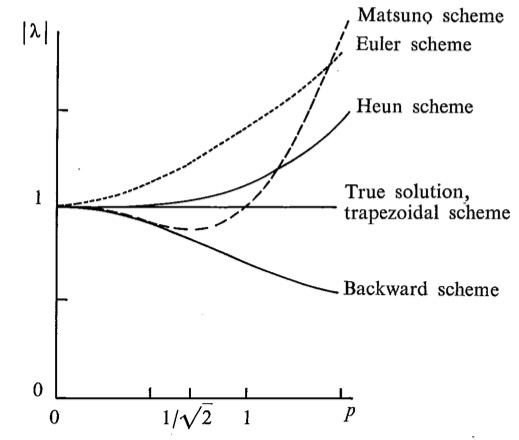
\includegraphics[width = .7 \textwidth]{figs/NM/pic5.jpg}
    \caption{} \label{fig:}
\end{figure}

Figure \texttt{figg:5} Summarizes the results obtained for the five
schemes considered so far. For all of these schemes the amplification
factors were found to be even functions of \(p\), so the amplification
factor curves are shown only for \(p \geq 0\).

It is also of interest to consider the phase change per time step,
\(\theta\) and the relative phase change per time step, \(\theta p\).

Using the notation

\[\lambda \equiv \lambda_{\text{re}} + i\lambda_{im}\]

we have, using \texttt{h2.4},

\[\theta = \arctan\frac{\lambda_{\text{im}}}{\lambda_{\text{re}}}\]

or

\[\frac{\theta}{p} = \frac{1}{p}\arctan\frac{\lambda_{\text{im}}}{\lambda_{\text{re}}}\]

For the Euler and the backward schemes, using \texttt{h2.11} and
\texttt{h2.12} we obtain

\[\frac{\theta}{p} = \frac{1}{p}\arctan\text{p}\]

Since the right-hand side is always less than unity, we can see that
these two schemes are decelerating. For \(p = 1\) we have
\(\theta p = \pi 4\).

In other cases the effect may not be so obvious. For the Matsuno scheme,
for example, \texttt{h2.21} gives

\[\frac{\theta}{p} = \frac{1}{p}\arctan\frac{p}{1 - p^{2}}\]

It is not obvious whether the right-hand side here is greater or less
than unity. However, the behaviour of \texttt{h2.31} for all \(p\) is of
no practical interest, since we already know that $p$ must be chosen
less than unity in order to ensure stability, and rather small for
frequencies for which we want the integration errors to be small. Thus,
we need only consider :eq:`h2.31 for small $p$; we obtain

\[\frac{\theta}{p} = 1 + \frac{2}{3}p^{2} + \ldots\]

The Matsuno scheme, therefore, is seen to be accelerating. For the
special value \(p = 1\) this can be seen directly from \texttt{h2.13},
since then \(\frac{\theta}{p} = \frac{\pi}{2}\).

Analysis of phase errors of schemes applied to the oscillation equation
is not so important as analysis of the amplification factor. Phase
errors do not affect stability, and when these schemes are used to solve
the partial differential equations of motion additional phase errors due
to space differencing will appear. We will then be interested only in
the total phase error, and it will be found that the error due to space
differencing is usually dominant.

\subsection{Three level schemes and computational
modes}\label{subsec:three-level-schemes-and-computational-modes}

We consider first the leapfrog scheme \texttt{h1.9}. Applied to the
oscillation equation it gives

\[U^{n + 1} = U^{( n + 1 )} + i 2\omega\Delta U^{\left( n \right)}\]

A problem with all three or more level schemes including this is that
they require more than one initial condition to start the computation.
From a physical standpoint a single initial condition
\(U^{\left( 0 \right)}\) should have been sufficient. However, in
addition to the physical initial condition, three level schemes require
a computational initial condition \(U^{\left( 1 \right)}\)). This value
cannot be calculated by a three level scheme, and, therefore, it will
usually have to be obtained using one of the two level schemes.

According to \texttt{h2.3} we also have

\[U^{\left( n \right)} = \lambda U^{\left( n - 1 \right)},
U^{\left( n + 1 \right)} = \lambda^{2}U^{\left( n - 1 \right)}\]

When these relations are substituted into \texttt{h2.32} we obtain

\[\lambda^{2} - i2p\lambda - 1 = 0\]

a second degree equation for \(\lambda\). It has solutions

\[\lambda_{1} = \sqrt{1 + p^{2}} + i p\]\[\lambda_{2} = - \sqrt{1 - p^{2}} + i p\]

Thus, there are \emph{two solutions} of the form
\(U^{n + 1} = \lambda U^{( n )}\). This necessarily follows from the
fact that we are considering a three level scheme; substitution of
\texttt{h2.33} into the difference equation given by these schemes will
always give a second degree equation for \(\lambda\). In general, an
\emph{m} level scheme will give $m-1$ solutions of the form
\(U^{n + 1} = \lambda U^{\left( n \right)}\). A solution of this type
corresponding to a single value of \(\lambda\) is called a \emph{mode}.

Consider now the two values that have been obtained for \(\lambda\). If
a solution of the form \(U^{n + 1} = \lambda U^{\left( n \right)}\) is
to represent an approximation to the true solution, then we must have
\(\lambda \rightarrow 1\) as \(\Delta \rightarrow 0\). For the values
\texttt{h2.34}, as \(p \equiv \omega\Delta t \rightarrow 0\) we do have
\(\lambda_{1} \rightarrow 1\), however at the same time
\(\lambda_{2} \rightarrow - 1\). Solutions like that associated with
\(\lambda_{2}\) are usually called \emph{physical modes} because we are
always solving equations describing physical processes. Solutions like
that associated with \(\lambda_2\) are not approximations to the true
solution, and are called \emph{computational modes}.

To clarify this situation we consider the simple case \(\omega = 0\),
that is, the equation

\[\frac{d U}{d t} = 0\]

with the true solution

\[U = const\]

The leapfrog scheme, applied to \texttt{h2.35}, gives

\[U^{\left( n + 1 \right)} = U^{\left( n - 1 \right)}\]

For a given physical initial condition \(U^{\left( 0 \right)}\), we
consider two special choices of \(U^{\left( 1 \right)}\).

A. Suppose calculating of \(U^{\left( 1 \right)}\) happened to give the
true value \(\text{U}^{\left( 0 \right)}\), \texttt{h2.37} then gives,
for all n,

\[U^{\left( n + 1 \right)} = U^{\left( n \right)}\]

or, since p = 0,

\[U^{\left( n + 1 \right)} = \lambda_{1}U^{\left( n \right)}\]

Thus, we obtain a numerical solution that is equal to the true solution
\texttt{h2.36}, and consists of the physical mode only.

B. Suppose calculating \(U^{\left( 1 \right)}\) gives
\(U^{\left( 1 \right)} = - U^{\left( 0 \right)}\).

Then we obtain, for all n,

\[U^{\left( n + 1 \right)} = - U^{\left( n \right)}\]

or

\[U^{\left( n + 1 \right)} = \lambda_{2}U^{\left( n \right)}\]

The numerical solution now consists entirely of the computational mode.
Hence, it would appear that a good choice of the computational initial
condition is of vital importance for obtaining a satisfactory numerical
solution.

In general, since \texttt{h2.31} is a linear equation, its solution will
be a linear combination of the two solutions

\[U_{1}^{\left( n \right)} = \lambda_{1}^{n}U_{1}^{\left( 0 \right)}\]\[U_{2}^{\left( n \right)} = \lambda_{2}^{n}U_{2}^{\left( 0 \right)}\]

Therefore, we can write

\[U^{\left( n \right)} = a\lambda_{1}^{n}U_{1}^{\left| 0 \right|} + b\lambda_{2}^{n}U_{2}^{\left( 0 \right)}\]

where a and b are constants. Now this has to satisfy the physical and
the computational initial condition; we obtain

\[U^{\left( 0 \right)} = a U_{1}^{\left| 0 \right|} + b U_{2}^{\left( 0 \right)}\]\[U^{\left( 1 \right)} = a\lambda_{1}U_{1}^{\left( 0 \right)} + b U_{2}^{\left( 0 \right)}\]

These equations can be solved for a \(U_{1}^{\left( 0 \right)}\) and
\(bU_{2}^{\left( 0 \right)}\), and the results substituted into
\texttt{h2.38}.

In this way we find

\[U^{(n)} = \frac{1}{\lambda_1 - \lambda_2} \left[ \lambda_1^n\left( U^{(1)}
- \lambda_{2}U^{(0)} \right) - \lambda_2^n\left( U^1 - \lambda_{1}U^{(0)} \right) \right]\]

Therefore, the amplitudes of the physical and of the computational modes
are seen to be proportional to, respectively,

\[|U^{(1)} - \lambda_2 U^{(0)}| \quad   and   \quad | U^{(1)} - \lambda_1 U^{(0)} |\]

These are seen to depend on \(U^{\left( 1 \right)}\). If, for example,
we are able to choose
\(U^{\left( 1 \right)} = \lambda_{1}U_{1}^{\left( 0 \right)}\), the
numerical solution will consist of the physical mode only. If, on the
other hand, the choice of \(U^{\left( 1 \right)}\) is so unsuccessful as
to have \(U^{\left( 1 \right)} = \lambda_{2}U^{\left( 0 \right)}\), the
solution will consist entirely of the computational mode.

While this analysis illustrates the importance of a careful choice of
\(\text{U}^{\left( 1 \right)}\), it is not always possible to calculate
\(U^{\left( 1 \right)} = \lambda_{1}U^{\left( 0 \right)}\) so as to
eliminate the computational mode. Numerical methods are used in practice
to solve equations that cannot be solved by analytical methods, and are
more complex than the simple oscillation equation \texttt{h2.1}. In
these cases we will not know the exact values of \(\lambda_{1}\) and
\(\lambda_{2}\).

Thus \(U^{\left( 1 \right)}\),, is usually computed using one of the two
level schemes. The simplest method is to use the Euler scheme, or, a
more refined procedure could be used, for example the Heun scheme. Using
\texttt{h2.39} it can be shown that the latter alternative will give a
smaller amplitude of the computational mode.

We also note that even if we did know the exact value of \(\lambda_{1}\)
this would still not allow the computational mode to be eliminated in a
practical numerical calculation. The numerical solution which we
calculate is not an exact solution of the finite difference equations,
since the arithmetical operations are performed in practice only to a
finite number of significant digits. The error produced in this way is
called \emph{round off error}, though in electronic computers results of
arithmetic operations are sometimes truncated to a given number of
digits, instead of being rounded off. With round off errors present,
permanent elimination of the computational mode is not possible in
principle, since the computational mode would appear in the course of
integration in any case even if were absent initially. However, it is
usually found that round off errors are of little importance in
atmospheric models, and in solving partial differential equations in
general.

Proceeding now to the stability analysis, in view of \texttt{h2.38} and
our inability to eliminate the computational mode completely, we will
have to require for stability that neither of the two amplification
factors is greater than unity. It is convenient to consider three
special cases.

\subsubsection{\(\left| p \right| \leq 1.\)}\label{subsubsec:p-smaller-1.}

In \texttt{h2.34} \(1 - p^{2}\) is positive, and we obtain
\(\left| \lambda_{1} \right| = \left| \lambda_{2} \right| = 1\)

Thus, in this case both modes are stable and neutral. For the phase
change, using \texttt{h2.28}

\[\theta_{1} = arctan\left( \frac{p}{\sqrt{1 - p^{2}}} \right)\]

\[\theta_{2} = arctan\left( \frac{- p}{\sqrt{1 - p^{2}}} \right)\]

It is instructive to consider the behaviour of \(\theta\), as a function
of \(p\), especially as \(p \rightarrow 0.\) We consider first the case
\(p > 0.\). Since for both modes
\(\lambda_{\text{im}} = \left| \text{λ} \right|\sin{\theta = p}`we
have :math:`0 < \theta < \pi\). Considering the signs of
\(\lambda_{\text{re}}`we find that,
:math:`0 < \theta < \frac{\pi}{2}`and
:math:\)frac\{pi\}\{2\} \textless{} t\href{}{heta}\{2\} \textless{} pi`.
To illustrate these results, the phase changes \texttt{h2.41} are
plotted in \texttt{figg:6}. We see that, for all \(p\),

\begin{figure}
    \centering
    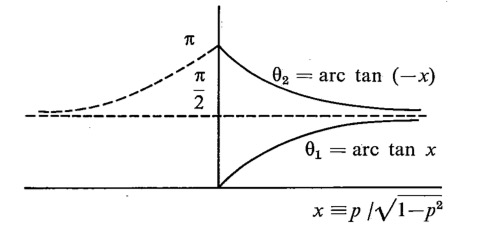
\includegraphics[width = .7 \textwidth]{figs/NM/pic6.jpg}
    \caption{} \label{fig:}
\end{figure}

\[\theta_{2} = \pi - \theta_{1}\]

Specifically, as \(p \rightarrow 0, \theta_{1} \rightarrow p\) while
\(\theta_{2} \rightarrow \pi - p\)

Thus, for small \(\Delta t\) the physical mode is seen to approximate
the true solution, while the behaviour of the computational mode is
quite different. For the case \(p < 0\), we obtain in the same way

\[\pm \theta_{2} = - \pi - \theta_{1}\]

Thus, for \(p \gtrless 0\)

\[\theta_{2} = \pm \pi - \theta_{1}\]

For accuracy of the physical mode, \(\theta_{1}\) should closely
approximate the phase change of the true solution, \emph{p}. For small
\emph{p} \texttt{h2.41} gives

\[\theta_{1} = p + \frac{1}{6}p^{3} + \ldots\]

Thus, the leapfrog scheme is accelerating. The acceleration, though, is
four times less than that of the Matsuno scheme. It is instructive to
note that schemes of different orders of accuracy can still have the
same order of leading term in power series expansions of either the
amplification factors or the phase changes.

Differentiating the first equation in \texttt{h2.41} we find

\[\frac{d\theta_{1}}{\text{dp}} = \frac{1}{\sqrt{1 - p^{2}}}\]

The phase error, thus, is seen to increase sharply as
\(p \rightarrow 1.\), when
\(\frac{\theta_{1}}{p} \rightarrow \frac{\pi}{2}\)

It may be useful to illustrate the behavior of the two modes obtained

\[
    U_{1}^{\left( n \right)}=
    U_{1}^{\left( 0 \right)}e^{in\theta 1}\]\[U_{2}^{\left( n \right)} =
    U_{2}^{\left| 0 \right|}e^{\text{in}\left( \pm \pi - \theta_{1} \right)}
\]

in the complex plane. For simplicity, we consider the case
\(\theta_{1} = \frac{\pi}{8}\) and assume that the imaginary part of the
solution is equal to zero at the initial moment. The physical mode, as
seen in \texttt{h2.43}, rotates in the positive sense by an angle
\(\theta_{1}\) in each time step \(\Delta t\), while at the same time
the computational mode, in the case \emph{p \textgreater{} 0}, rotates
by an angle \(\pi - \theta_{1}\). Therefore, the two modes can be
represented graphically as in \texttt{figg:7}.

\begin{figure}
    \centering
    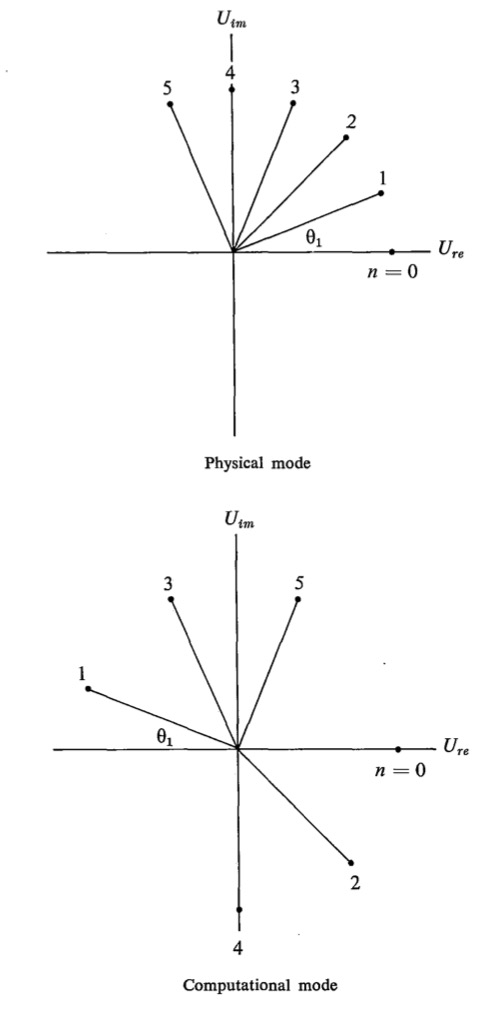
\includegraphics[width = .7 \textwidth]{figs/NM/pic7.jpg}
    \caption{} \label{fig:}
\end{figure}

A detailed knowledge of the behaviour of the computational mode may be
helpful in recognizing its excessive presence in an integration. Thus,
we plot the real and imaginary parts of the computational mode as
functions of time. This can be done by using an alternative form of the
second equation in \texttt{h2.43}

\[U_{2}^{\left( n \right)} = {\left( - 1 \right)^{n}U}_{2}^{\left( 0 \right)}\left( \cos{n\theta_{1}} - i\sin{n\theta_{2}} \right)\]

or directly from \texttt{figg:7}. We obtain diagrams as shown in
\texttt{figg:8}. Because of the factor $(-1)^n$, both real and imaginary
parts oscillate between time steps.

\begin{figure}
    \centering
    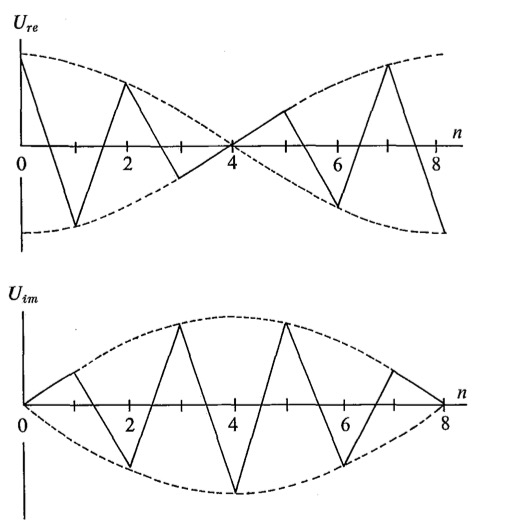
\includegraphics[width = .7 \textwidth]{figs/NM/pic8.jpg}
    \caption{} \label{fig:}
\end{figure}

\subsubsection{\(\left| p \right| = 1\)}\label{subsubsec:left-p-right-1}

This is a limiting case of the solutions considered for
\(\left| \text{p} \right| < 1\). \texttt{h2.34} shows that the values of
\(\lambda\). are now equal,

\[\lambda_{1} = 2 = ip\]

Therefore

\[\left| \lambda_{1} \right| = \left| \lambda_{2} \right| = 1\]

Thus, both modes are still neutral. Since neither of them has a real
part, we obtain, for p = ± 1,

\[\theta_{1} = \theta_{2} = \pm \frac{\pi}{2}\]

Therefore, the two modes can be written in the form

\[U^{\left( n \right)} = U^{\left( 0 \right)}e^{\pm i n\frac{\pi}{2}}\]

In a complex plane, they rotate by an angle of \(\frac{\pm \pi}{2}\) in
each time step, while the true solution rotates by an angle of ± 1
only. The phase error, thus, is large.

\subsubsection{\(\left| p \right| > 1\)}\label{subsubsec:p-greater-1}

Both values of \(\lambda\) in \texttt{h2.34} still have imaginary parts
only, so that

\[\lambda_{1} = i\left( p + \sqrt{p^{2}} - 1 \right)\]\[\lambda_{2} = i\left( p - \sqrt{p^{2} - 1} \right)\]

where the expressions in parentheses are real. Therefore,

\[\left| \lambda_{1} \right| = \left| p + \sqrt{p^{2}} - 1 \right|\]\[\left| \lambda_{2} \right| = \left| p - \sqrt{p^{2}} - 1 \right|\]

Thus, for $p > 1$ we have
\(\left| \lambda_{1} \right| > 1\), and for $p< 1$
\(\left| \lambda_{2} > 1 \right|\). Therefore, for
\(\left| p > 1 \right|\) the leapfrog scheme is unstable. The
instability increases sharply as \(\left| \text{p} \right|\) increases
beyond 1 ; we can see this, for example for \emph{p \textgreater{} 1},
because

\[\frac{d\left| \lambda \right|_{1}}{\text{dp}} = 1 + \frac{p}{\sqrt{p^{2}} - 1}\]

which is unbounded as \(p \rightarrow 1\)

Since the two values of \(\lambda\) still have no real parts, we again
have

\[\theta_{1} = \theta_{2} = \pm \frac{\pi}{2}\]

The two modes for \(p \gtrless 1\), can thus be written as

\[U_{1}^{\left( n \right)} = \left| p + \sqrt{p^{2} - 1} \right|^{n}U_{1}^{\left( 0 \right)}e^{\pm in\frac{\pi}{2}}\]\[U_{2}^{\left( n \right)} = \left| p - \sqrt{p^{2} - 1} \right|^{n}U_{2}^{\left( 0 \right)}e^{\pm in\frac{\pi}{2}}\]

In the complex plane, both modes again rotate by an angle of
\(\frac{\pm \pi}{2}\) in each time step. However, this time the
amplitude of one of the modes increases, and that of the other decreases
with time. The real part of the unstable mode can, for instance, be
represented as a function of time by a graph like that in Fig. 2.5.
Because of \texttt{h2.48} the period of the unstable oscillation is
always \(4\Delta t\). This can be used to diagnose the instability: if
the results appear unsatisfactory, it is a good idea to

check for the presence of growing oscillations of that period.

\begin{figure}
    \centering
    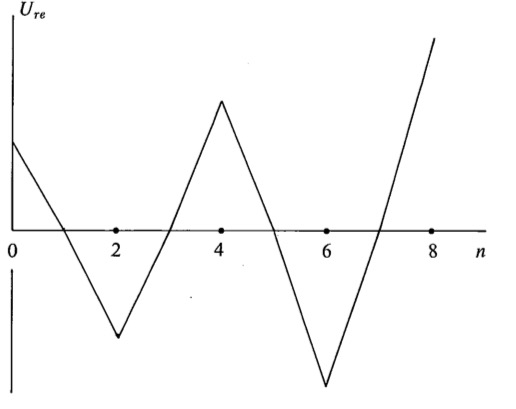
\includegraphics[width = .7 \textwidth]{figs/NM/pic9.jpg}
    \caption{} \label{fig:}
\end{figure}

To sum up, advantages of the leapfrog scheme are that it is a very
simple scheme, of second order accuracy, and neutral within the
stability range \(\left| \omega\Delta t \leq 1 \right|\). A disadvantage
of the leapfrog scheme is the presence of a neutral computational mode.
With nonlinear equations there is a tendency for a slow amplification of
the computational mode. An example of this growth can be seen, for
example, in one figure of a paper by Lilly (1965). The usual method used
for suppressing this instability is the occasional insertion of a step
made by a two level scheme, which eliminates the computational mode. A
multi-level scheme that damps the computational mode could also be used
for this purpose.

When solving the system of gravity wave equations, as will be shown in
Chapter \texttt{Chapter4}, it is possible to construct grids and/or
finite difference schemes which have essentially the same properties as
the leapfrog scheme, but in which the computational mode is absent.
These methods calculate the physical mode only, and at the same time
require only one half of the computation time needed for the regular
leapfrog scheme as described here.

We consider, finally, stability and other properties of the
Adams-Bashforth scheme \texttt{h1.10}. Applied to the oscillation
equation it gives

\[U^{( n + 1 )} = U^{(n)} + i\omega\Delta t \left( \frac{3}{2}U^{( n )} - \frac{1}{2}U^{\left( n - 1 \right)} \right)\]

Substituting the relations \texttt{h2.33} we find

\[\lambda^{2} - \left( 1 + i\frac{3}{2}p \right)\lambda + i\frac{1}{2}p = 0\]

We have, of course, again obtained a second degree equation for
\(\lambda\).

It has the solutions

\[\lambda_{1} = \frac{1}{2}\left( 1 + i\frac{3}{2}p + \sqrt{1 - \frac{9}{4}p^{2} + ip} \right)\]\[\lambda_{2} = \frac{1}{2}\left( 1 + i\frac{3}{2}p - \sqrt{1 - \frac{9}{4}}p^{2} + ip \right)\]

Thus, as \(p \rightarrow 0\), \(\lambda_{1} \rightarrow 1 \) while
\(\lambda_{2} \rightarrow 0\). We see that the solution associated with
\(\lambda_{2}\) again represents a physical mode, and that associated
with \(\lambda_{2}\) a computational mode. However, while for the
leapfrog scheme the computational mode was found to be neutral, here it
is seen to be damped. This is a very useful property of the
Adams-Bashforth scheme as the computational mode cannot cause
inconveniences.

The exact analysis of the amplification factors here is more difficult
because of the presence of square roots in \texttt{h2.51}. However,
since for reasons of accuracy we have to choose a relatively small value
of p in any case, it will suffice to consider amplification factors for
small values of p only. The power series expansion of \texttt{h2.51}
then gives

\[\lambda_{1} = 1 + ip - \frac{1}{2}p^{2} + i\frac{1}{4}p^{3} - \frac{1}{8}p^{4} + \ldots\]\[\lambda_{2} = i\frac{1}{2}p^{2} + i\frac{1}{2}p^{2} - \frac{1}{4}p^{3} + \frac{1}{8}p^{4}\ldots\]

Now, after rearranging the terms these series can be written as

\[\lambda_{1} = \left( 1 - \frac{1}{2}p^{2} - \frac{1}{8}p^{4} - \ldots \right) + i\left( p + \frac{1}{4}p^{3} + \ldots \right)\]\[\lambda_{2} = \left( \frac{1}{2}p^{2} + \frac{1}{8}p^{4} + \ldots \right) + i\left( \frac{1}{2}p - \frac{1}{4}p^{3} - \ldots \right)\]

which can be used to obtain the amplification factors

\[\left| \lambda_{1} \right| = \left( 1 + \frac{1}{2}p^{4} + \ldots \right)^{\frac{1}{2}}\]\[\left| \lambda_{2} \right| = \left( \frac{1}{4}p^{2} + \ldots \right)^{\frac{1}{2}}\]

The higher order terms have been omitted. A final expansion gives

\[\left| \lambda_{1} \right| = 1 + \frac{1}{4}p^{4} + \ldots\]\[\left| \lambda_{2} \right| = \frac{1}{2}p + \ldots\]

Expressions \texttt{h2.52} and/or \texttt{h2.53} show that the physical
mode of the Adams-Bashforth scheme is always unstable. However, as for
the Heun scheme, the amplification is only by a fourth order term, and
it can be tolerated when a sufficiently small value of \(\Delta t\) is
chosen. Note that the amplification given by \texttt{h2.53} is twice
that given by \texttt{h2.26} for the Heun scheme. Since the
amplification is proportional to \(\left( \Delta t \right)^{4}\),
however, a small reduction in time step would compensate for that
difference. Thus, the Adams-Bashforth scheme, with only one evaluation
of the right hand side per time step, can still be considered much more
economical. It has been fairly frequently used in meteorological
numerical studies. For example, it is being used by Deardorff in his
numerical simulations of the planetary boundary layer (e.g. Deardorff,
1974).

Analyses of the properties of some other schemes, applied to the
oscillation equation, can be found in papers by Lilly (1965), Kurihara
(1965) and Young (1968). In practice the choice of a scheme will depend
not only on the properties considered here, but also on some practical
considerations. For example, we might expect that the three level
schemes, since they use more information, would generally give better
results than the two level schemes. Our findings agree with that
conjecture ; for example, for second order accuracy the explicit three
level schemes required only one evaluation of the right hand side per
time step, while the two level schemes required two evaluations. As
another example, if we want to damp high frequency motions with three
level schemes we can linearly extrapolate the derivative beyond the
centre of the interval
\(\left( n\Delta t,\left( n + 1 \right)\Delta t \right)\), and thus
obtain a scheme that will perform such a damping in a more selective and
more economical way than the Mat-suno scheme (Mesinger, 1971). However,
three level schemes generally require more core storage space in the
computer than two level schemes and this may affect our our decision.

\section{Properties of schemes applied to the friction equation}
\label{sec:properties-of-schemes-applied-to-the-friction-equation}

We shall now consider the properties of schemes when applied to the
equation

\[\frac{d U}{d t} = - \kappa U, \qquad U = U\left( t \right), \qquad \kappa > 0\]

We shall call this equation the friction equation.

Again it is easy to justify our interest in this equation. For example,
if we define \(U \equiv u + iv\), it describes the effect of friction
proportional to the velocity vector, as is often assumed for motions
near the ground. As another example, note that when seeking a solution
of the heat transfer, or Fick\textquotesingle s diffusion equation

\[\frac{\partial u}{\partial t} = \sigma\frac{\partial^{2} u }{{\partial x}^{2}}, \qquad \sigma > 0\]

in the form of a single harmonic component

\[u\left( x,t \right) = Re\left\lbrack \left( U\left( t \right)e^{\text{ikx}} \right) \right\rbrack\]

we obtain

\[\frac{\text{dU}}{\text{dt}} = - \sigma k^{2}U\]

\begin{description}
    \item[This is equivalent to \texttt{k3.1} if we substitute]
    \(x \equiv \sigma k^{2}\).
\end{description}

The general solution of \texttt{k3.1} is

\[U\left( t \right) = U\left( 0 \right)e^{- \kappa t}\]

Thus, both the real and the imaginary part decrease exponentially with
time.

The properties of schemes applied to \texttt{k3.1} will again be
analyzed using the von Neumann method. As in the previous section, we
consider first the non-iterative two level scheme \texttt{h2.6}. Applied
to the friction equation, \texttt{h2.6} gives

\[U^{(n + 1)} = U^{n} - \kappa\Delta t \left( \alpha U^{( n )} + \beta U^{\left( n + 1 \right)} \right)\]

Writing

\[K \equiv \kappa \Delta t\]

we obtain, rearranging the terms in \texttt{k3.3},

\[U^{\left( n + 1 \right)} = \frac{1 - \alpha K}{1 + \beta K}U^{\left( n \right)}\]

For the Euler scheme \(\alpha = 1`and :math:\)beta = 0`; thus,
\texttt{k3.5} shows that the Euler scheme is now stable if
\(\left| 1 - K \leq 1 \right|\), that is, if

\[0 < K \leq 2\]

Thus we see that the stability criteria of particular schemes do not
have to be the same when they are applied to different equations. In the
case of \texttt{k3.6}, one will normally be more demanding in the choice
of \(\Delta t\). For example, we will want \emph{K \textless{} 1}, to
prevent the solution \texttt{k3.5} oscillating from time step to time
step.

For the backward scheme \(\alpha = 0`and :math:\)beta = 1`; it is always
stable if \emph{K \textgreater{} 0}. The solution does not oscillate in
sign.

For the trapezoidal scheme \(\alpha = \frac{1}{2}`and
:math:\)beta = frac\{1\}\{2\}`; the scheme is again always stable for
\emph{K \textgreater{} 0}. The solution does not oscillate if \emph{K
\textless{} 2}.

Considering the iterative two level scheme \texttt{h2.18} we obtain

\[U^{\left( n + 1 \right)} = \left( 1 - K + \beta K^{2} \right)U^{\left( n \right)}\]

Therefore, both the Matsuno and the Heun scheme are stable for
sufficiently small values of \emph{K}.

It is instructive to consider in some detail the behaviour of the
numerical solution obtained using the leapfrog scheme. Applied to
\texttt{k3.1} it gives

\[U^{\left( n + 1 \right)} = U^{\left( n - 1 \right)} - 2\Delta t U^{\left( n \right)}\]

The equation for the amplification factor is

\[\lambda^{2} + 2K\lambda - 1 = 0\]

giving the solutions

\[\lambda_{1} = - K + \sqrt{1 + K^{2}}\]\[\lambda_{2} = - K - \sqrt{1 + K^{2}}\]

As \(k \rightarrow 0, \quad \lambda \rightarrow 1,\) while
\(\lambda_{2} \rightarrow - 1\) thus, the solution associated with
\(\lambda_{1}\) again represents the physical mode, and that associated
with \(\lambda_{2}\) the computational mode. For \emph{K \textgreater{}
0}, that is, for the normal case of a forward integration in time, we
have \(\lambda_{2} < - 1\); hence, the computational mode is always
unstable. It changes sign from time step to time step, and its magnitude
increases. As before, we cannot hope to eliminate the computational
mode completely. This amplification is not negligible, and the leapfrog
scheme is therefore not suitable for numerical integration of the
friction equation.

A simple example can be given to illustrate the instability of the
leapfrog scheme. Let U have only a real part, and suppose we have set
\(U^{( 1 )} = U^{( 0 )}\), as shown in \texttt{figg:10} Furthermore, let
the dashed curve in the figure represent the true solution satisfying
the given initial condition \(U^{\left( 0 \right)}\). Knowing
\(U^{\left( 0 \right)}\), \(U^{\left( 1 \right)}\), and the true
solution it is possible to construct a graph of the numerical solution,
using the fact that \(\frac{\text{dU}}{dt = - \kappa U}\) is equal to
the slope of the line tangent to the true solution at the appropriate
value of U. In this way we obtain the numerical solution shown by the
full line. In this method, the derivative is calculated as a function
of the current value of \(U^{\left( n \right)}\), and the increment due
to this derivative is added to the preceding value. This is seen to
result in an unbounded growth of the difference between consecutive
values of \(U^{\left( n \right)}\), even when this difference is equal
to zero initially.

\begin{figure}
    \centering
    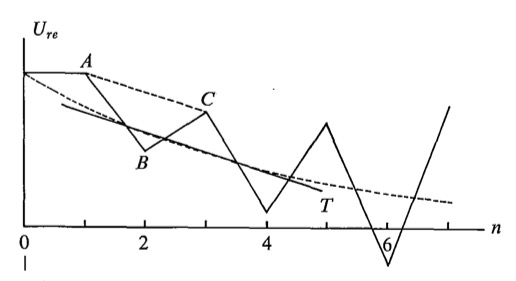
\includegraphics[width = .7 \textwidth]{figs/NM/pic10.jpg}
    \caption{} \label{fig:}
\end{figure}

Finally, for the Adams-Bashforth scheme we obtain

\[\lambda = \frac{1}{2}\left( 1 - \frac{3}{2}K \pm \sqrt{1 - K\frac{9}{4}K^{2}} \right)\]

The Adams-Bashforth scheme, thus, is stable for sufficiently small
values of K. The computational mode is damped.

\section{A combination of schemes}\label{sec:combination-of-schemes}

A natural question to ask at this point is what can we do if, for
example, the equation contains both the oscillation and the friction
term, that is

\[\frac{\text{dU}}{\text{Dt}} = i\omega U - \kappa U\]

Here we might like to use the leapfrog scheme because of the oscillation
term \(i\omega U\), but we know that it cannot be used for the friction
term \(- \kappa U\). In this and similar situations we can use different
schemes for the different terms; for example, we might use the leapfrog
scheme for the oscillation term and the forward scheme for the friction
term. We then obtain

\[U^{\left( n + 1 \right)} = U^{\left( n - 1 \right)} + 2\Delta t\left( i\omega U^{\left( n \right)} - \kappa U^{\left( n - 1 \right)} \right)\]

Other combinations, of course, are also possible.